\section{Localization}

Localization mechanisms:

\begin{description}
		\item[Coordinate systems] Absolute (global), relative (to local point, known by full network), local (to commmunicating parties)
		\item[Algorithms] Centralized, distributed, localized
		\item[Measurement parameters] Distances (lateration), angles (angulation)
		\item[Range-free vs range-based] Range-measurements, using eg received
				signal strength for distance estimation. Range-free, using
				connectivity information (lower accuracy, lower hardware
				requirements)
\end{description}


\subsection{Distance estimation}

\subsubsection{Time of arrival}

Distance $d = ((T_3 - T_0) - (T_2 - T_1)) \cdot v / 2$.
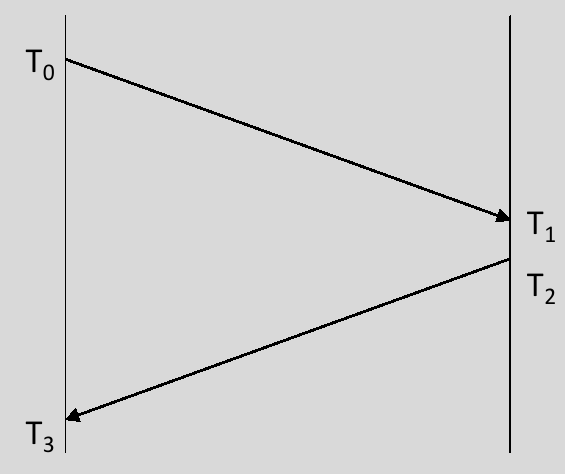
\includegraphics[width=0.5\textwidth]{04_time_of_arrival}

Example: Time-of-flight sensor network ranging.

\subsubsection{Time difference of arrival}

Transmission of two different signals from a single point. Either to same
source (two signal types, eg ultrasound and radio waves), or to two landmarks.
Signal transmission time irrelevant. Each measurement defines a hyperbola,
intersection of two provides a fixed distance (but not position!).

Distance $d = ((T_3 - T_1) - (T_2 - T_0)) \cdot (v_1 \cdot v_2) / (v_1 - v_2)$.

Example: Cricket.

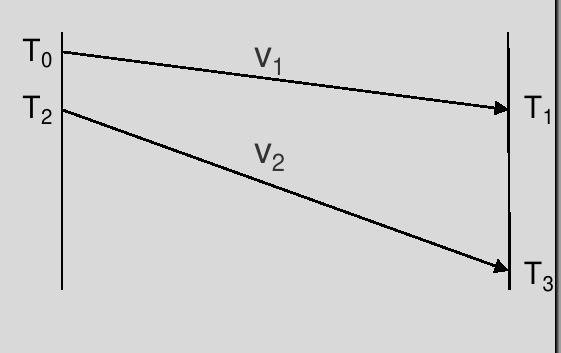
\includegraphics[width=0.5\textwidth]{04_time_difference_of_arrival}

\subsubsection{RSSI}

$PL$ path loss, $d_0$ nearby reference point, $n$ loss coefficient. Then $PL(d)
= PL(d_0) + 10 \cdot n \cdot \log(\frac{d}{d_0})$.

Problem: Unstable path loss / distance curve due to environmental conditions.

\subsubsection{Lighthouse location system}

Assumption: Parallel beam of width $b$ transmitted from lighthouse. Each node
measures time $t_{beam}$ it saw the beam. $t_{turn}$ time for beam to do one
rotation. Then:

\begin{align*}
		d = \frac{b}{2 \cdot \sin(\pi \cdot \frac{t_{beam}}{t_{turn}})}
\end{align*}

Problem: Parallell beam might be hard to realize, but can be improved with two
lighthouses.

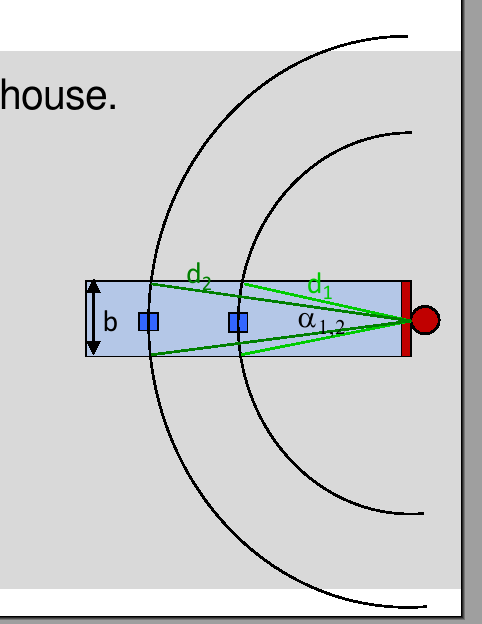
\includegraphics[width=0.5\textwidth]{04_lighthouse}

\subsection{Angle estimation}

Can be done using directional antennas, or phase/time difference of signal
arrival from multiple antennas.

\subsubsection{Beam forming}

Directional antenna allows detecting direction of signal, and hence angle to
signal source.

\subsubsection{VHS omni-directional ranging}

Landmark sends two signals: One periodic and omni-directional with period $p$,
one directional and rotating. Node measures time difference $d$ between first
and second signal, then $\alpha = d / p \cdot 2 \pi$.

\subsubsection{RSS estimation}

Ratio of RSS between two directional antennas depends on angle of signal.

\subsubsection{Compass}

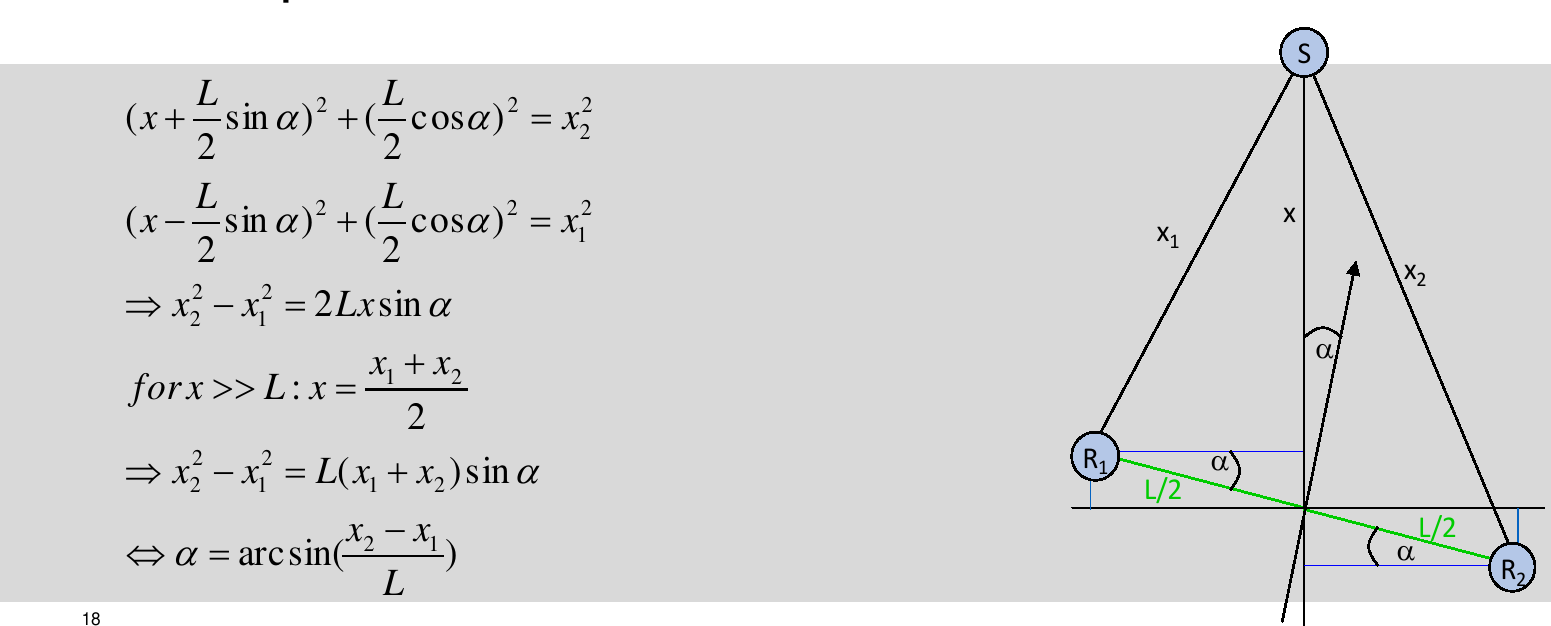
\includegraphics[width=0.8\textwidth]{04_compass}

\subsection{Range-based localization}

\subsubsection{Bounding box}

Boxes around anchor nodes where distance is known. Intersection of boxes is
bounding box for location.

\subsubsection{Weighted centroid}

Set of anchor nodes with known positions $x_i$. Weights $\omega_i$ dependant on
eg number of beacons from node, RSSI, etc. Then position:
\begin{align*}
		x = \frac{\sum_{i = 1}^N \omega_i \cdot x_i}{\sum_{i = 1}^N \omega_i}
\end{align*}

\subsubsection{Trilateration \& multilateration}

Distance measuremetns to landmark nodes. Curves have intersections, 3
measurements for position in plane (assuming everyone on ground!). Errors can
cause an area instead of a single point, redundant measurements with
least-squares compensation can help.

Multilateration extends by using >3 landmark nodes. Given distances $d_i$ to
nodes with positions $(x_i, y_i$), linearization of the $(x_i - x)^2 + (y_i -
y)^2 = d_i^2$. Then solving overdetermined system with e.g. least-squares.

\subsubsection{Triangulation}

Nodes measure angles to landmarks. Circles denote points with same angle to two
points, node must then lie oncircle intersections.

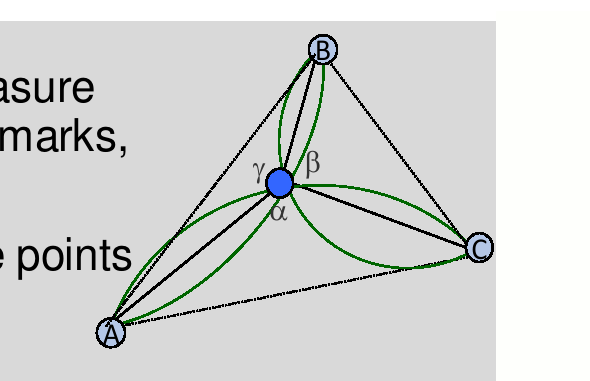
\includegraphics[width=0.5\textwidth]{04_triangulation}

\subsubsection{Fingerprinting}

Comparison of received signal patterns with database. Requires offline
collection phase where signals from base stations at various positions
measured. Then on-line phase where e.g. nearest-neighbour-signal-space
minimizes distance to known DB entries. Optionally use average of closest $k =
2, 3, 4$ DB entries as position.

\subsection{Range-free localization}

Techniques based on information of network area (eg overlapping transmission
ranges), hop count, neighbours, ...

\subsubsection{Approximate point in triangle}

Node detects whether inside or outside of triangles of its neighbours. Node
must then be in intersection of triangles it is within.

If node able to move: Perfect triangulation test possible by moving node. If
inside triangle, moving any direction will bring you closer to at least one
corner, and farther from at least one corner. If outside triangle, there must
exist a direction where it gets closer to, or farther from, all corners.

Otherwise, approximate point-in-triangulation test by estimating distance from
neighbours using eg RSSI. If any of its neighbours is closer/farther than
itself from all corners, its neighbour (and by assumption the node itself) must
be outside. Otherwise, its neighbour (and the node itself) inside the triangle.

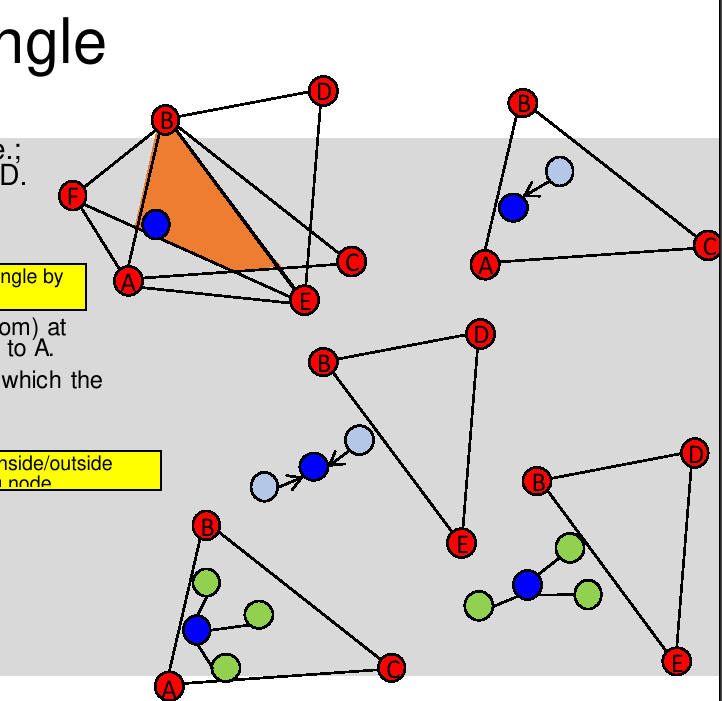
\includegraphics[width=0.6\textwidth]{04_approximate_point_in_triangle}

\subsection{Localization in multi-hop environments}

Nodes adjacent to landmarks estimate their position. Neighbours use nodes with
known positions as landmarks.

\subsubsection{Ad-hoc positioning system}

\begin{itemize}
		\item Node connected to landmark learns distance
		\item Nodes with neighbours who know their distance compute their own
				distance to the landmark, by using their distance to these
				nodes. Example: $B, C$ known distance to $L$. $A$ knows
				distance to $B, C$, allowing it to compute distance to $L$.
\end{itemize}

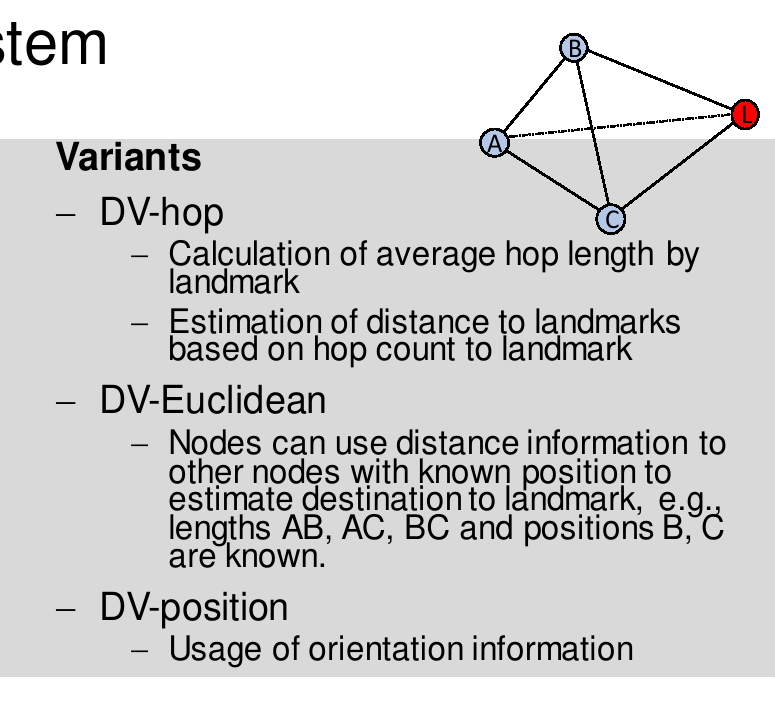
\includegraphics[width=0.6\textwidth]{04_adhoc_positioning}

\subsubsection{Ad-hoc localization}

\begin{itemize}
		\item Nodes learning their position via landmarks act as landmarks for other nodes
		\item Problem: If node not adjacent to more than 2 landmarks, not possible
		\item Approach: Have nodes collaborate to find groups where sufficient
				equations present to solve system
\end{itemize}
